\section{Pair folding and resolving batches}
\label{sec:folding}

Identifying pairs of vertices reduces the order of the graph to which
induction will be applied. After setting aside loops and all but one edge
in each parallel class, each quotient edge has a unique original
representative. A quotient cycle may enter a pair at one member and leave
through the other; a reserved path joins them. To obtain a simple cycle,
the interiors of these paths must avoid all representative endpoints and
be pairwise disjoint within that cycle.

The first lemma bounds the number of edges set aside in this cleanup.
A degree bound at the paired vertices alone is insufficient: for positive
integers $a$ and $m$ with $m$ even, pairing the $m$-vertex side of
$K_{m,a}$ forces $am/2$ edges to be set aside, although each paired vertex
has degree $a$. The lemma therefore also bounds the number of neighbors
in each folding set at every vertex, including vertices outside those sets.

\begin{lemma}[Pair folding]\label{lem:pair-folding}
Let $J$ be a finite simple graph and let $X_1,\ldots,X_t$ be pairwise
disjoint subsets of its vertex set.  Suppose that $a\ge1$, that
$m_i=\abs{X_i}\ge\max\{8,a^2\}$ for every $i$, and that
\begin{align}
 d_J(x)&\le a &&\text{for every }x\in\bigcup_i X_i,\label{eq:fold-degree}\\
 d_i(v):=\abs{N_J(v)\cap X_i}&\le a
     &&\text{for every }v\in V(J)\text{ and every }i.
     \label{eq:fold-neighbors}
\end{align}
There are pairings within the $X_i$, each leaving exactly $m_i\bmod2$
vertices unpaired, and a set $E_{\rm err}\subseteq E(J)$ with
\[
 \abs{E_{\rm err}}\le 2\sum_i m_i,
\]
such that identifying each pair in $J-E_{\rm err}$ gives a simple graph
$Q$.  Every edge of $Q$ has exactly one retained original edge as its
representative.  Retaining all quotient vertices, including isolated ones,
we have
\begin{equation}\label{eq:fold-order}
 \abs{V(Q)}=\abs{V(J)}-\sum_i\floor{m_i/2}.
\end{equation}
The assertion also holds when the family of folding sets is empty.
\end{lemma}

\begin{proof}
Choose a uniform perfect pairing when $m_i$ is even.  When $m_i$ is odd,
adjoin a dummy vertex, choose a uniform perfect pairing on the $m_i+1$
vertices, and delete the dummy vertex and its incident pairing edge,
leaving its original partner unpaired.  Each pairing with
one unpaired original vertex has exactly one extension of this kind, so
the resulting distribution is uniform.  Make the choices for different
$i$ independently.

For distinct specified vertices $u,v$ of a set of order $m$, symmetry of
the partner of $u$ gives the following exact probabilities.  For two
prescribed disjoint pairs, conditioning on the first pair leaves a uniform
perfect pairing on the remaining vertices, including the dummy when
present.  Thus
\begin{equation}\label{eq:fold-probabilities}
\begin{array}{c|cc}
 &m\text{ even}&m\text{ odd}\\ \hline
 \Pr(\{u,v\}\text{ is a pair})
     &\dfrac1{m-1}&\dfrac1m\\[6pt]
 \Pr(\text{two prescribed disjoint pairs occur})
     &\dfrac1{(m-1)(m-3)}&\dfrac1{m(m-2)}
\end{array}
\end{equation}
In particular the even-column expressions are valid upper bounds for
both parities.

Let $\pi$ send each vertex to its fiber after the identifications.  Every
fiber has size one or two.  Before removing any edges, let $Z$ count the
original edges that become loops, plus the unordered pairs of distinct
original edges that become the same nonloop edge.  We bound $\E Z$ by
classifying all possible errors.

\paragraph{Loops and collisions with a common original endpoint.}
An original edge becomes a loop precisely when its endpoints form a pair
in some $X_i$.  There are at most $a m_i/2$ original edges inside $X_i$,
so its expected loop contribution is at most $a m_i/(2(m_i-1))$.

Two distinct edges sharing an original endpoint have the form $vu,vw$
with $u\ne w$.  If they become the same nonloop edge, then
$\pi(u)=\pi(w)\ne\pi(v)$, so $u,w$ must be paired in some $X_i$.
No other identification is possible: identifying all three original
vertices would require a fiber of size at least three.  Consequently the
contribution charged to $X_i$ is at most
\[
 \frac1{m_i-1}\sum_{v\in V(J)}\binom{d_i(v)}2
 \le \frac{a(a-1)m_i}{2(m_i-1)}.
\]
Here $\binom d2\le(a-1)d/2$ for every integer $0\le d\le a$, and
\[
 \sum_{v\in V(J)}d_i(v)=\sum_{x\in X_i}d_J(x)\le a m_i.
\]
The equality counts both incidences of every internal edge on both sides.
Combining the loop and common-endpoint bounds, the expectation is at most
\begin{equation}\label{eq:fold-first-errors}
 \sum_i\frac{a^2m_i}{2(m_i-1)}
 \le\frac47\sum_i a^2,
\end{equation}
since $m_i\ge8$.

\paragraph{Collisions with four distinct original endpoints.}
Write the two edges as $uv$ and $xy$, with four different vertices.
For them to become the same nonloop edge, the two fibers must be either
$\{u,x\},\{v,y\}$ or $\{u,y\},\{v,x\}$.  All four vertices therefore
belong to folding sets: a singleton fiber cannot contain two distinct
original endpoints.  If the two paired fibers lie in one $X_i$, then both
original edges are internal to $X_i$.  Writing $e_i=\abs{E(J[X_i])}$,
there are at most $\binom{e_i}2\le e_i^2/2$ possible vertex-disjoint edge
pairs, and the two possible
pairing patterns give probability at most
$2/((m_i-1)(m_i-3))$.  As $e_i\le a m_i/2$, their total contribution is
at most
\begin{equation}\label{eq:fold-internal-errors}
 \sum_i\frac{a^2m_i^2}{4(m_i-1)(m_i-3)}
 \le\frac{16}{35}\sum_i a^2.
\end{equation}
For the last inequality use $m_i/(m_i-1)\le8/7$ and
$m_i/(m_i-3)\le8/5$.

If the two paired fibers instead lie in different sets $X_i,X_j$, then
both original edges run between those sets.  There is just one possible
pairing pattern, since each pair must remain within its own set.  Put
$e_{ij}=e_J(X_i,X_j)$; there are at most $\binom{e_{ij}}2\le e_{ij}^2/2$
vertex-disjoint edge pairs.  Independence between the two pairings and
\eqref{eq:fold-probabilities} bound this contribution by
\begin{align}
 \sum_{i<j}\frac{e_{ij}^2}{2(m_i-1)(m_j-1)}
 &\le\frac{32}{49}\sum_{i<j}\frac{e_{ij}^2}{m_i m_j}
 \le\frac{16}{49}\sum_i a^2.\label{eq:fold-cross-errors}
\end{align}
Indeed, for each fixed $i$,
\[
 \sum_{j\ne i}\frac{e_{ij}^2}{m_i m_j}
 \le\frac a{m_i}\sum_{j\ne i}e_{ij}\le a^2:
\]
the first inequality uses $e_{ij}\le a m_j$, and the second follows from
the total degree bound on $X_i$.  Summing over $i$ counts each unordered
pair of sets twice.  The preceding cases exhaust distinct original
edges, which either have one common endpoint or have four distinct
endpoints in a simple graph.

Equations \eqref{eq:fold-first-errors}--\eqref{eq:fold-cross-errors} give
\[
 \E Z\le
 \left(\frac47+\frac{16}{35}+\frac{16}{49}\right)\sum_i a^2
 =\frac{332}{245}\sum_i a^2
 \le\frac{332}{245}\sum_i m_i<2\sum_i m_i
\]
when $t>0$.  Some choice of pairings has no greater error count than its
expectation.  For this choice delete each original loop edge and, in each
nonloop parallel class of size $s$, delete all but one original edge.
The latter requires $s-1\le\binom s2$ deletions, so the number of deleted
edges is at most $Z$.  The remaining graph is simple after identification,
and the retained representative in each class is unique.  Deletions do
not remove vertices, giving \eqref{eq:fold-order}.  If $t=0$, use the
identity map and delete no edges.
\end{proof}

The next lemma resolves all batches within a single earlier box.  Its
hypotheses keep the degree bound global over those batches.  Different
batches may contain the same vertex and may pair that vertex differently;
their original edge sets are disjoint.

\begin{lemma}[Batch resolution]\label{lem:batch-resolution}
For every sufficiently large real $D$, set
\[
 a=D^{0.01},\qquad L_0=D^{0.03},\qquad
 B_0=D^{0.30},\qquad \sigma=D^{0.90}.
\]
Let $Y$ be a finite vertex set.  Let $\mathcal W$ be a finite indexed
family of subsets $W\subseteq Y$, with $\abs W\le B_0$, and let $J_W$
be a simple graph on $W$ for each index.  Suppose these graphs have
pairwise disjoint edge sets, and let $F=F(Y)$ be their union, taken on
$Y$.

Let $\mathcal R$ be a family of simple graphs on pairwise disjoint vertex
subsets of $Y$.  Suppose that each $R\in\mathcal R$ has order
$\sigma\le r_R\le D^{1.02}$, that
$E(R)\cap E(F)=\varnothing$, and that its edges are partitioned into
two spanning graphs $P_R,T_R$, both of cut expansion at least
$\sigma/4$.  Call $P_R$ the router.

For some pairs $(W,R)$ let an active set
$X_{W,R}\subseteq W\cap V(R)$ be specified, satisfying
\begin{equation}\label{eq:batch-active-hypotheses}
 \abs{X_{W,R}}\ge L_0,
 \qquad d_F(x)\le a\quad(x\in X_{W,R}).
\end{equation}
Sums over $(W,R)$ below include only active sets, and write
$\Sigma_Y=\sum_{W,R}\abs{X_{W,R}}$.

There are finite simple quotient graphs $Q_W$, with all quotient vertices
retained, whose orders satisfy
\begin{align}
 q_W&=\abs W-\sum_{R:\,(W,R)\text{ active}}
                 \floor{\abs{X_{W,R}}/2}\notag\\
 &\le\abs W-\frac13
            \sum_{R:\,(W,R)\text{ active}}\abs{X_{W,R}}
 \le B_0,\label{eq:batch-quotient-order}\\
 \sum_W q_W&\le\sum_W\abs W-\frac13\Sigma_Y.
 \label{eq:batch-total-order}
\end{align}
For every choice of cycle-and-edge partitions of these $Q_W$, having
$t_W$ parts, there are sets $U_R\subseteq E(P_R)$ and a cycle-and-edge
partition of
\[
 E(F)\mathbin{\dot\cup}\mathop{\dot\bigcup}_{R\in\mathcal R}U_R
\]
with at most
\begin{equation}\label{eq:batch-parts}
 \sum_W t_W+8\Sigma_Y
\end{equation}
parts.  The graphs $R'=R-U_R$, kept on $V(R)$, contain the untouched
spanning graphs $T_R$, so each still has a spanning subgraph of cut
expansion at least $\sigma/4$.  The completed parts and these remaining
graphs together partition
$E(F)\mathbin{\dot\cup}\mathop{\dot\bigcup}_{R\in\mathcal R}E(R)$.
All thresholds in this lemma are absolute.
\end{lemma}

\begin{proof}
We first choose the quotient graphs and prepare some paths to be closed.
No router edges are used until all quotient partitions have also been
specified.

\paragraph{Removing edges to heavy neighbors.}
The path trimming below is the elementary operation used by
Conlon, Fox and Sudakov~\cite[Lemma~6.3]{CFS2014}: decompose a
bipartite graph into paths and remove terminal edges so that the
remaining endpoints lie on one prescribed side. We keep the endpoint
loads under the single degree bound on the union of all batches.
Fix a batch $W$.  Its active sets are pairwise disjoint because the pieces
$R$ have disjoint vertex sets.  For an active set $X=X_{W,R}$ put
\[
 H_X=\{v\in W:\abs{N_{J_W}(v)\cap X}>a\},
 \qquad E_X=E_{J_W}(X,H_X).
\]
Every vertex in any active set has degree at most $a$ in $J_W$, since
$J_W\subseteq F$.  Thus $H_X$ is disjoint from every active set in this
batch, including $X$.  If $H_X$ is nonempty, counting edges gives
\[
 a\abs{H_X}<\abs{E_X}
 \le\sum_{x\in X}d_{J_W}(x)\le a\abs X;
\]
in all cases $\abs{H_X}\le\abs X$.  The sets $E_X$ for different active
$X$ are disjoint.  In fact each of their edges has one endpoint in its
specified active set and its other endpoint outside every active set,
so it cannot belong to the set specified by a different active set.

Apply \Cref{cor:endpoint-paths} to the bipartite graph with parts
$X,H_X$ and edge set $E_X$.  It gives at most
$\abs X+\abs{H_X}\le2\abs X$ positive-length simple paths, since their
total number of endpoint occurrences is at most
$2(\abs X+\abs{H_X})$.  From each path delete its terminal
edge at each endpoint belonging to $H_X$, counting those deleted edges
singly.  At most two distinct edges are deleted.  A one-edge path has
only one endpoint in $H_X$, and if both endpoints lie in $H_X$, the
path has at least two edges, with distinct terminal edges.

Ignore any remnant with no edges.  Every other remnant is a simple path
with both endpoints in $X$: this follows directly by removing the
$H_X$ endpoints from the alternating bipartite path.  Its length is
even and at least two, so its endpoints are distinct.  For each such
remnant $L$ record a demand between its endpoints in $P_R$, forbid
internally the set $V(L)\cap V(R)$, and give this demand its own team.
Once this demand is routed, its remnant will form one cycle.  Each
original path therefore accounts for at most two single edges and one
cycle, for a total of at most $6\abs X$ parts.  We do not require an
endpoint-load-two bound for the trimmed paths; their endpoint loads will
be bounded using their incident original edges in the global load
argument below.

\paragraph{Choosing the quotients.}
Remove all the sets $E_X$ from $J_W$ and call the resulting graph $J_W^0$,
retaining the vertex set $W$.  Each active vertex still has degree at
most $a$.  For each active $X$ and every $v\in W$, either $v$ was in
$H_X$, in which case all its edges into $X$ were removed, or it originally
had at most $a$ neighbors in $X$.  Hence
$\abs{N_{J_W^0}(v)\cap X}\le a$ in both cases.
For large $D$ we have $L_0\ge\max\{8,a^2\}$.  Apply
\Cref{lem:pair-folding} to $J_W^0$ and its active sets.  Count its error
edges singly in their original form and call the simple resulting
quotient $Q_W$.  Denote its quotient map by $\pi_W$; each edge $e$ of
$Q_W$ has a unique retained original representative $\widehat e$.
The number of these single-edge parts is at most
$2\sum_R\abs{X_{W,R}}$.

Every identified pair removes exactly one vertex.  Since
$\floor{m/2}\ge m/3$ for every integer $m\ge2$, the exact order formula
from \Cref{lem:pair-folding} yields
\eqref{eq:batch-quotient-order}, and summing yields
\eqref{eq:batch-total-order}.  This construction of all $Q_W$ is
independent of their subsequent partitions.

\paragraph{The switch demands of a quotient cycle.}
Now fix arbitrary cycle-and-edge partitions of all the $Q_W$.  Restore
each single-edge part as its unique original representative.  For a
cycle $C$ in $Q_W$, list its distinct vertices in cyclic order as
$z_1,\ldots,z_s$, where $s\ge3$, and write $e_j=z_jz_{j+1}$, with
indices interpreted cyclically.  At $z_j$ let $u_j$ be the endpoint of
$\widehat e_{j-1}$ in the fiber $\pi_W^{-1}(z_j)$, and let $v_j$ be
the endpoint of $\widehat e_j$ in that fiber.  If $u_j=v_j$, the two
edges join without any added path.  Otherwise that fiber is a folded
pair $\{u_j,v_j\}$ in one active set $X_{W,R}$; record a demand from
$u_j$ to $v_j$ in $P_R$.

For every demand from this cycle forbid internally
\[
 Z_C\cap V(R),\qquad
 Z_C=\bigcup_{j=1}^s V(\widehat e_j).
\]
Thus every original endpoint on the entire cycle, including the
endpoints of all its other switches, is forbidden internally.  The
demands belonging to this cycle and this router form one team.  Teams
for different cycles, including cycles from different batch indices,
are distinct.  The single-demand teams recorded during the heavy-neighbor
work are also distinct from these teams.
Figure~\ref{fig:cycle-lifting} shows the switch construction. The
next two steps verify that all these requested paths can be chosen
simultaneously and that the resulting closed walks are simple.

\begin{figure}[tbp]
\centering
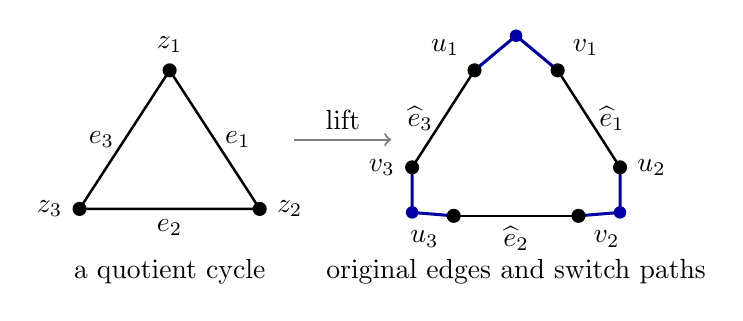
\begin{tikzpicture}[x=0.88cm,y=0.88cm,
  original/.style={line width=0.9pt},
  route/.style={line width=1.1pt,blue!65!black},
  vertex/.style={circle,fill=black,inner sep=1.8pt},
  inside/.style={circle,fill=blue!65!black,inner sep=1.6pt}]
\coordinate (z1) at (0,1.8);
\coordinate (z2) at (1.3,-0.2);
\coordinate (z3) at (-1.3,-0.2);
\draw[original] (z1)--node[right] {$e_1$}(z2)--node[below] {$e_2$}(z3)--node[left] {$e_3$}(z1);
\node[vertex,label=above:$z_1$] at (z1) {};
\node[vertex,label=right:$z_2$] at (z2) {};
\node[vertex,label=left:$z_3$] at (z3) {};
\node at (0,-1.1) {a quotient cycle};
\draw[->,gray,thick] (1.8,0.8)--(3.2,0.8);
\node[above] at (2.5,0.8) {lift};
\coordinate (u1) at (4.4,1.8);
\coordinate (v1) at (5.6,1.8);
\coordinate (u2) at (6.5,0.4);
\coordinate (v2) at (5.9,-0.3);
\coordinate (u3) at (4.1,-0.3);
\coordinate (v3) at (3.5,0.4);
\draw[original] (v1)--node[right] {$\widehat e_1$}(u2);
\draw[original] (v2)--node[below] {$\widehat e_2$}(u3);
\draw[original] (v3)--node[left] {$\widehat e_3$}(u1);
\draw[route] (u1)--(5,2.3)--(v1);
\draw[route] (u2)--(6.5,-0.25)--(v2);
\draw[route] (u3)--(3.5,-0.25)--(v3);
\node[inside] at (5,2.3) {};
\node[inside] at (6.5,-0.25) {};
\node[inside] at (3.5,-0.25) {};
\node[vertex,label=above left:$u_1$] at (u1) {};
\node[vertex,label=above right:$v_1$] at (v1) {};
\node[vertex,label=right:$u_2$] at (u2) {};
\node[vertex,label=below right:$v_2$] at (v2) {};
\node[vertex,label=below left:$u_3$] at (u3) {};
\node[vertex,label=left:$v_3$] at (v3) {};
\node at (5,-1.1) {original edges and switch paths};
\end{tikzpicture}
\caption{Lifting a quotient cycle, schematically. The fiber at \(z_j\)
contains \(u_j,v_j\); when they differ, a reserved path (blue) joins
them. The black edges are the unique original representatives of the
quotient edges. Every path interior avoids all black-edge endpoints,
and the interiors are pairwise disjoint for this cycle. Each blue
path is drawn with one internal vertex only for illustration; its
actual length may differ. A visit with \(u_j=v_j\) requires no path.}
\label{fig:cycle-lifting}
\end{figure}



\paragraph{The load bound over all batches.}
Fix one piece $R$.  Gather every demand for $P_R$ from all batches and
both constructions.  Each endpoint is in an active set, hence has
degree at most $a$ in the one graph $F(Y)$.  To bound its total demand
load, associate each occurrence of an endpoint $x$ with an incident
edge of $F(Y)$ as follows:
\begin{itemize}
 \item For the demand closing a remnant $L$, use the terminal edge of
       $L$ at $x$.
 \item At a switch $u_j\ne v_j$, associate the occurrence of $u_j$
       with $\widehat e_{j-1}$ and that of $v_j$ with $\widehat e_j$.
\end{itemize}
At a fixed vertex these associated incident edges are distinct.  For
the first construction this follows from the edge-disjoint path
partition and from the disjointness of the designated edge sets.
For the second construction a quotient edge belongs to exactly one
part, has exactly one original representative, and its incidence at a
given original vertex can be used only at the unique visit to its
quotient fiber in that cycle.  The cycles are simple, and a switch uses
different original vertices for its two incidences.  The two constructions
use disjoint edges because all designated edges were removed before
folding.  Finally, edges from different batches are distinct by
hypothesis, regardless of overlap of their vertex sets or differences
in their pairings.  This proves the injection into incident edges of
$F(Y)$ and hence
\begin{equation}\label{eq:batch-global-load}
 \text{number of demand-end occurrences at }x
 \le d_{F(Y)}(x)\le a.
\end{equation}
Vertices that are never endpoints have load zero.

\paragraph{Supplying all the connections.}
A team from a cycle $C$ has at most $s\le q_W\le B_0$ demands, and
$\abs{Z_C}\le2s\le2B_0$.  A heavy-neighbor remnant has at most
$\abs W\le B_0$ vertices; its team has size one.  Thus in
\Cref{lem:routing} we may use
\[
 r=r_R,\qquad h=\sigma/4,\qquad
 k=a,\qquad b=B_0,\qquad z=2B_0.
\]
With that lemma's definitions of $g$ and $\ell$, the range
$\sigma\le r_R\le D^{1.02}$ gives, uniformly in $R$,
\[
 \ell=O(D^{0.12}\log^2 D),
 \qquad
 \ell^2(a+B_0)+2B_0
       =O(D^{0.54}\log^4 D)=o(D^{0.90}).
\]
For all sufficiently large $D$ this is at most $\sigma/256=h/64$,
which is exactly enough for \eqref{eq:routing-condition}.  Apply the
routing lemma once to this full collection in $P_R$; if the collection
is empty, use no edges.  The paths supplied are pairwise edge-disjoint
over all teams and all batches for this $R$, and their internal vertex
sets are pairwise disjoint within each team.  Do this for every piece
$R$.  The constants are absolute, and do not depend on the number of
batches or demands.

\paragraph{Simplicity of the completed cycles.}
For a heavy-neighbor remnant $L$, its supplied path is simple and has
distinct endpoints equal to those of $L$.  Its internal vertices avoid
$V(L)$: the forbidden set contains $V(L)\cap V(R)$, and all supplied
path vertices lie in $V(R)$.  The union
is therefore a simple cycle.  It has at least two remnant edges and at
least one supplying edge, so its length is at least three.

For a quotient cycle $C$, the fibers of $z_1,\ldots,z_s$ are mutually
disjoint.  At a visit with $u_j=v_j$, its original representative edges
use one vertex.  At a switch, they use the two different vertices of
that fiber and the supplied simple path joins them.  Thus before
adding path interiors, the vertices at different visits are distinct.
Every supplying path interior avoids $Z_C$, which includes all these
original vertices.  Two supplying paths for this cycle in the same
router have disjoint interiors by their common team; paths in different
routers lie in the disjoint vertex sets of different pieces $R$.
Consequently interiors of any two switches are disjoint, and none
contains an endpoint of another switch or any other original vertex
used by the cycle.  Traversing the representatives and these connections
in cyclic order therefore visits no vertex twice, except the start
when closing the cycle.

An unused twin deserves explicit mention.  If a visited fiber is a pair
but $u_j=v_j$, its other vertex need not belong to $Z_C$ and may occur
inside a supplying path.  It is absent from all original representative
edges of this cycle, since those edges use distinct fibers.  If it is
used internally, no second supplying path of this cycle can use it:
the team condition excludes this in its router, and the other routers
have disjoint vertex sets.  This therefore creates no repeated vertex.
The same reasoning covers vertices in fibers not visited by the cycle.

The resulting cycle contains its $s$ distinct original representative
edges and possibly additional edges, so its length is at least
$s\ge3$.  A quotient cycle with no switches is already a simple cycle
of original edges.  Each quotient part thus yields exactly one permitted
part.

\paragraph{Edge accounting and cost.}
For each batch, its original edges have exactly four destinations:
\begin{enumerate}
 \item designated edges trimmed from paths are single-edge parts;
 \item designated edges in positive-length remnants occur in their
       closed cycles;
 \item folding error edges are single-edge parts, taken before
       identification;
 \item retained edges have unique representatives in $Q_W$ and occur
       once in the restored quotient parts.
\end{enumerate}
These classes partition $E(J_W)$.  Empty remnants leave no unaccounted
edge, and the deletion rule for parallel classes retains exactly one
representative for each quotient edge.  Since the $J_W$ have disjoint
edge sets, every edge of $F$ occurs once in this list over all batches.

Let $U_R$ be the set of edges used by all supplying paths in $P_R$.
Each is used once by the routing lemma.  These edges are disjoint from
$E(F)$ by hypothesis, and different routers have disjoint edge sets.
Thus all completed parts form an edge partition of the edge set in the
statement.  The heavy-neighbor work contributes at most $6\Sigma_Y$
parts, folding errors at most $2\Sigma_Y$, and the quotient partitions
contribute exactly $\sum_W t_W$.  Adding a supplying path changes no
part count.  This proves \eqref{eq:batch-parts}.

No edge of $T_R$ was used: $U_R\subseteq E(P_R)$ and $E(P_R)$ is
disjoint from $E(T_R)$.  Therefore $R'=R-U_R$ contains the entire
spanning graph $T_R$ on its original vertex set.  The edges of $R'$
are precisely the edges of this assigned piece not already used in a
completed part.  This proves both the remaining expansion assertion
and the final edge partition.
\end{proof}
